%% Standalone figure: compile this file once (pdflatex lorentz.tex) to produce lorentz.pdf,
%% which main.tex includes with \includegraphics. Recompile only after editing the figure.
\documentclass[11pt,tikz,border=2pt]{standalone}
\usepackage{amsmath,amssymb}       % \text, \vec, math symbols
\usetikzlibrary{arrows.meta}       % Stealth arrow tips
\begin{document}
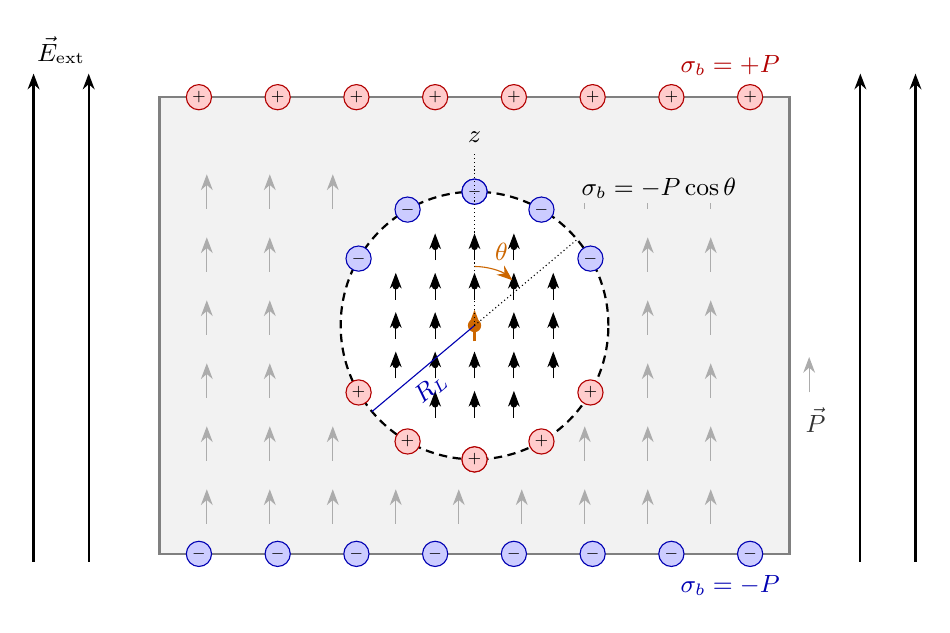
\begin{tikzpicture}[
  font=\small,
  >={Stealth[length=2mm]},
  negcharge/.style={circle, draw=blue!70!black, fill=blue!20, inner sep=0pt, minimum size=3.2mm},
  poscharge/.style={circle, draw=red!70!black,  fill=red!20,  inner sep=0pt, minimum size=3.2mm},
]
  \def\RL{1.7}     % Lorentz sphere radius R_L (cm)
  \def\W{4.0}      % half width of the sample (cm)
  \def\H{2.9}      % half height of the sample (cm)

  % ---------- external field outside the sample ----------
  \foreach \X in {-5.6,-4.9,4.9,5.6}{
    \draw[->, thick] (\X,-3.0) -- (\X,3.2);
  }
  \node[anchor=south] at (-5.25,3.2) {$\vec E_{\text{ext}}$};

  % ---------- polarized sample (continuum outside the sphere) ----------
  \fill[gray!10] (-\W,-\H) rectangle (\W,\H);
  \draw[thick, gray] (-\W,-\H) rectangle (\W,\H);
  \foreach \x in {-3.4,-2.6,...,3.4}{
    \foreach \y in {-2.3,-1.5,...,2.4}{
      \pgfmathsetmacro{\d}{sqrt(\x*\x+\y*\y)}
      \pgfmathtruncatemacro{\out}{\d > \RL+0.35}
      \ifnum\out=1 \draw[->, gray!65] (\x,\y-0.22) -- (\x,\y+0.22); \fi
    }
  }
  \node[anchor=west, gray!40!black] at (\W+0.08,-1.2) {$\vec P$};
  \draw[->, gray!65] (\W+0.25,-0.85) -- (\W+0.25,-0.40);

  % ---------- bound charge on the outer surface ----------
  \foreach \x in {-3.5,-2.5,...,3.5}{
    \node[poscharge] at (\x,\H) {\tiny$+$};
    \node[negcharge] at (\x,-\H) {\tiny$-$};
  }
  \node[anchor=south east, red!70!black] at (\W,\H+0.15) {$\sigma_b = +P$};
  \node[anchor=north east, blue!70!black] at (\W,-\H-0.15) {$\sigma_b = -P$};

  % ---------- Lorentz sphere (imaginary cavity) ----------
  \fill[white] (0,0) circle (\RL);
  \draw[thick, densely dashed] (0,0) circle (\RL);
  % cavity surface charge sigma_b = -P cos(theta): negative on top, positive at the bottom
  \foreach \t in {0,30,60}{
    \node[negcharge] at ({\RL*sin(\t)},{\RL*cos(\t)}) {\tiny$-$};
    \node[negcharge] at ({-\RL*sin(\t)},{\RL*cos(\t)}) {\tiny$-$};
    \node[poscharge] at ({\RL*sin(\t)},{-\RL*cos(\t)}) {\tiny$+$};
    \node[poscharge] at ({-\RL*sin(\t)},{-\RL*cos(\t)}) {\tiny$+$};
  }
  \node[anchor=south west, fill=gray!10, inner sep=1.5pt] at (1.3,1.55) {$\sigma_b = -P\cos\theta$};

  % discrete dipoles inside the sphere (cubic lattice)
  \foreach \x in {-1.0,-0.5,...,1.0}{
    \foreach \y in {-1.0,-0.5,...,1.0}{
      \pgfmathsetmacro{\d}{sqrt(\x*\x+\y*\y)}
      \pgfmathtruncatemacro{\in}{(\d < \RL-0.45) && (\d > 0.01)}
      \ifnum\in=1
        \fill[black] (\x,\y) circle (1.2pt);
        \draw[->, black] (\x,\y-0.17) -- (\x,\y+0.17);
      \fi
    }
  }
  % central atom
  \fill[orange!80!black] (0,0) circle (2.4pt);
  \draw[->, thick, orange!80!black] (0,-0.2) -- (0,0.2);

  % radius and polar angle
  \draw[blue!70!black] (0,0) -- (-140:\RL) node[pos=0.55, below, sloped] {$R_L$};
  \draw[densely dotted] (0,0) -- (0,\RL+0.5) node[anchor=south] {$z$};
  \draw[densely dotted] (0,0) -- (40:\RL);
  \draw[->, orange!80!black] (0,0.75) arc (90:50:0.75);
  \node[orange!80!black] at (70:1.0) {$\theta$};
\end{tikzpicture}
\end{document}
